
\section{はじめに}
% \red{グラフ上の警邏問題を考えるにあたって,既存の結果との関連など}

1人または複数の巡査が所与の領域を動き回り,その領域内のあらゆる場所を十分な頻度で訪問することで,
これを守備,監督することを警邏(patrolling)という~\cite{czyzowicz2011boundary}.

警邏に関する研究には様々な問題設定があり,
例えば線分や閉路のような交わりの無い1次元的な領域のすべての点を警邏する
塀の警邏(Fence Patrolling)問題~\cite{chen2013fence, czyzowicz2011boundary}や,
より一般的なグラフで辺全体ではなく頂点を警備する警邏問題を考えることもできる~\cite{coene2011charlemagne}.
グラフと巡査が与えられて警邏可能かを判定する問題だけでなく,
塀の警邏問題においてなるべく長い塀を警邏する問題~\cite{czyzowicz2011boundary}や
全体の訪問の待ち時間の最大値を最小化する問題~\cite{chen2013fence}
% 頂点の警邏問題においては警備できる頂点数を最大化したり,
% 頂点に利得も設定して警備される頂点から得られる利得の合計を最大化する問題,
% {\timelimit}が頂点ごとに異なる場合~\cite{coene2011charlemagne}
なども考えられている.

Coeneら~\cite{coene2011charlemagne}は,
辺の長さの与えられた無向グラフと
各頂点の持つ利得・{\timelimit},巡査の人数が与えられたとき,
グラフの辺上を速さ1以下で動く1人または複数の巡査が,
各頂点を訪問する間隔をその頂点の{\timelimit}以内にしなければならない制約を満たしながら訪問し続けることで警備するとき,
警備される頂点の利得の合計を最大化するような頂点部分集合を求める警邏問題を考えた.
しかし,Coeneらは巡査が複数の場合もどの頂点も高々1人の巡査により警備される
(ある頂点を複数の巡査が協力して警備することはしない)という仮定を加えていた.

本稿ではこの問題を取り上げ,
複数の巡査が協力して警備する頂点があってもよいという設定で同じ問題を考える.
NP困難性や多項式時間アルゴリズムを示すのが難しかった部分については,
{\timelimit}の代わりに「{\period}」を考え,
頂点を最初に訪問した時刻からちょうど{\period}ごとの時刻にその頂点は訪問されなければならないという問題や,
さらに最初の訪問時刻も与えられる問題を考えて計算量クラスの評価を試みる.



\section{問題設定の詳細}
辺の長さの与えられた無向グラフの辺上を
点で表される1人または複数人の巡査が速さ1以下で動きながら頂点を訪問する.
各頂点には{\timelimit}が与えられている.
%
ある頂点を警備できているとは,どの連続した2回の訪問も間隔がその頂点の{\timelimit}以内となるように
訪問し続けられることと定義する.
また,訪問とは点で表される巡査が頂点を踏むことである.
巡査は2人以上同時に1つの頂点に存在してもよいし,
1つの頂点は複数人の巡査により交代で訪問して警備してもよい.
%
グラフと巡査の人数が与えられたときに,
グラフの全点を警備できるかを判定する問題を \decisionpp と呼び,
さらに各頂点に利得も与えられたときに警備される頂点から得られる利得の合計の最大値を求める
より一般的な問題を{\optpp}と呼ぶことにする.
こちらでは利得が $0$ 以下のものは警備する必要がないので最初に除外して利得はすべて正の整数であるとする.
{\timelimit}は非負整数とする.





\section{既存の結果との関連}
Coeneらは,グラフの形状として
Line(線分),Circle(閉路),Star(星),Tree(木),完全グラフ
を扱っていた~\cite{coene2011charlemagne}.
Lineは全ての頂点がある1つの線分上に存在するグラフ,
CircleはLineの両端をつなぐ辺を足したグラフである.
%
Line, StarはTreeの特殊な場合となる.
Lineは両端を結ぶ十分長い辺を足すことでCircleに帰着される.
完全グラフはその一部の辺を同様に十分長くすることで一般のグラフを表現できる.
%
巡査が1人の場合,Line, Circleでは多項式時間アルゴリズムが存在する一方,
Star, Treeでは利得と{\timelimit}がすべて等しい場合のみ多項式時間アルゴリズムが存在し,
いずれかが一般の場合はNP困難となり,
完全グラフ(一般のグラフ)ではNP困難となることが示されている.
%
巡査が複数の場合,
Line, Circleでは多項式時間アルゴリズムが存在し,Star以上ではNP困難となることが示されているが,
これは頂点の警備を巡査が協力して行わないという仮定の下での結果であった.
%

今回は巡査の協力も許す場合を考えるという目的で,
より単純なグラフであるLineと辺の長さがすべて等しい完全グラフ(以降{\comp}と呼ぶ)を扱うことにする.
%


\section{Line}

グラフがLineの場合は実直線上にすべての頂点を置くことができるので,
それぞれの座標を左端から順に$x_1, x_2, \ldots, x_n$とする.
巡査達の最高速度は皆同じなので,
巡査がすれ違うような動きはお互いの動きを交換し引き返すことで,
巡査は初期配置の$x$軸上の順番を保って動くとしてよいことが言える.
以降はこのような初期配置の順番を保つ動きのみを考える.



% \timelimit}がすべて等しい場合
まず,{\timelimit}がすべて等しい場合は{\optpp}に多項式時間アルゴリズムが存在する.
%
全点の{\timelimit}を$Q$,巡査の人数を$m$とするとき,
$n$個の各頂点に対応する
区間$[x_1, x_1 + Q/2], \ldots, [x_n, x_n + Q/2]$を考え,
それぞれの区間に含まれる頂点のもつ利得の合計が大きいものから$m$人の巡査がそれぞれ1つずつ区間を選び
この範囲を往復する動きが最適であることを示すことができるので,
動的計画法により$O(n \log n + nm)$時間で利得の最大値を求めることができる(詳細略).
%
この証明ではLineには端の頂点が存在することが重要な役割を果たしているので
Circleにそのまま適用することはできない.



% {\timelimit}が一般の場合
{\timelimit}がすべて等しい場合は
どの頂点も複数の巡査の協力で警備する必要がないので単純になっていたが,
%
{\timelimit}が一般の場合は,
ある{\timelimit}が短い頂点を複数の巡査が交代で訪問することで警備するのが
最適となるような例が存在する.
%
図\ref{tikz:multiserver_example2}は
横軸を頂点の位置,縦軸を時刻として$t$-$x$平面に巡査の軌跡を書いたものであるが,
%
左から{\timelimit}が$8,2,2,3,6$である5つの頂点
が存在するとき,
左図のような動きを繰り返せば
中央の{\timelimit}の短い頂点を協力して警備することで全点を警備できる.
左の巡査は{\timelimit}が$8$である頂点をより短い時間$6$ごとに訪問しているが,
このようにあえて早めに戻る動きをすることで右の巡査との協力が効率よくなっており,
仮に{\timelimit}ぎりぎりまで右の方へ動き頂点をなるべく多く訪問して帰るような戦略をとると
右図のようにどうしても訪問間隔が{\timelimit}を超え警備できない頂点が生まれてしまう.
%
この例は,協力が発生する場合巡査の動きを個々に決定するのが難しいことを示唆している.
%

\begin{figure}[h]
	\centering
	\begin{tabular}{cc}

	\begin{minipage}{0.5\hsize}
		\centering
		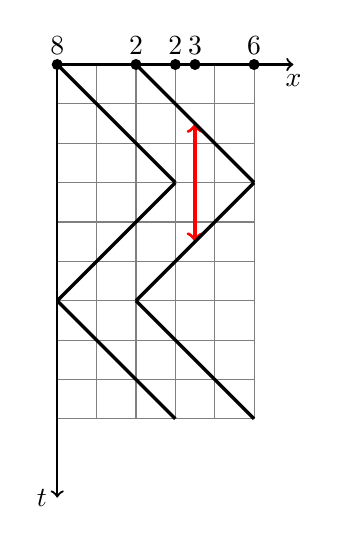
\begin{tikzpicture}
			\draw [help lines,thin,step=5mm] (0,-4.5) grid (2.5,0);
			\draw[thick, ->] (0,0) -- (3,0) node [below] {$x$};
			\draw[thick, ->] (0,0) -- (0,-5.5) node [left] {$t$};

			\fill ( 0   , 0) coordinate (c1) circle (2pt) node [above] {8};
			\fill ( 1   , 0) coordinate (c2) circle (2pt) node [above] {2};
			\fill ( 1.5 , 0) coordinate (c3) circle (2pt) node [above] {2};
			\fill ( 1.75, 0) coordinate (c4) circle (2pt) node [above] {3};
			\fill ( 2.5 , 0) coordinate (c5) circle (2pt) node [above] {6};

			\draw[very thick,red,<->] (1.75,-0.75)--(1.75,-2.25);

			\draw[very thick,-] ( 0  , 0  )--( 1.5,-1.5);
			\draw[very thick,-] ( 1.5,-1.5)--( 0  ,-3  );
			\draw[very thick,-] ( 0  ,-3  )--( 1.5,-4.5);
			\draw[very thick,-] ( 1  , 0  )--( 2.5,-1.5);
			\draw[very thick,-] ( 2.5,-1.5)--( 1  ,-3  );
			\draw[very thick,-] ( 1  ,-3  )--( 2.5,-4.5);
		\end{tikzpicture}
	\end{minipage}

	\begin{minipage}{0.5\hsize}
		\centering
		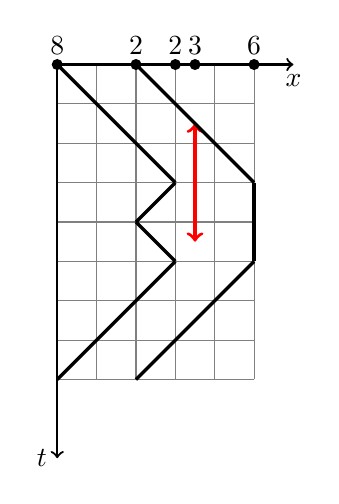
\begin{tikzpicture}
			\draw [help lines,thin,step=5mm] (0,-4) grid (2.5,0);
			\draw[thick, ->] (0,0) -- (3,0) node [below] {$x$};
			\draw[thick, ->] (0,0) -- (0,-5) node [left] {$t$};

			\fill ( 0   , 0) coordinate (c1) circle (2pt) node [above] {8};
			\fill ( 1   , 0) coordinate (c2) circle (2pt) node [above] {2};
			\fill ( 1.5 , 0) coordinate (c3) circle (2pt) node [above] {2};
			\fill ( 1.75, 0) coordinate (c4) circle (2pt) node [above] {3};
			\fill ( 2.5 , 0) coordinate (c5) circle (2pt) node [above] {6};

			\draw[very thick,red,<->] (1.75,-0.75)--(1.75,-2.25);

			\draw[very thick,-] ( 0  , 0  )--( 1.5,-1.5);
			\draw[very thick,-] ( 1.5,-1.5)--( 1  ,-2  );
			\draw[very thick,-] ( 1  ,-2  )--( 1.5,-2.5);
			\draw[very thick,-] ( 1.5,-2.5)--( 0  ,-4  );

			\draw[very thick,-] ( 1  , 0  )--( 2.5,-1.5);
			\draw[very thick,-] ( 2.5,-1.5)--( 2.5,-2.5);
			\draw[very thick,-] ( 2.5,-2.5)--( 1  ,-4  );
		\end{tikzpicture}
	\end{minipage}

	\end{tabular}
	\caption{巡査の協力が必要な例 \label{tikz:multiserver_example2}}
	% 「可能な限り右に手伝いに行く」戦略が失敗する例
\end{figure}


そこで我々は
{\timelimit}の代わりに「{\period}」というものを考え
{\period}ちょうどごとの時刻に訪問しなければならない問題も考えた.
この「あえて短い間隔で訪問する」ことで得をしにくいような設定では,
さらに各頂点について最初の訪問時刻も指定されるならば
できる限り右の方へ動く戦略で最適解が得られることを示すことができる.





\section{\comp}


% 完全グラフの場合は巡査が1人でもNP困難であることが示されていたので
{\comp}は辺の長さがすべて等しい完全グラフであるが,これはStarより簡単な図形という位置づけとなる.
実際,与えられた{\comp}の辺の長さを$d$としたとき,同じ頂点数で辺の長さが$d/2$であるStarを考えると
どちらも任意の2頂点間の移動距離が$d$である図形となり今回の問題設定では同等となる.
Starの結果から{\comp}も
巡査1人で利得と{\timelimit}がすべて等しい場合は{\optpp}を多項式時間で解くことができることがすぐに分かるが,
さらに{\timelimit}さえすべて等しければ巡査が複数で利得が一般の場合でも
{\optpp}を解く多項式時間アルゴリズムを示すことができる.
%
% {\timelimit}がすべて等しいときのアルゴリズム?
これは,警備のコストとなる辺の長さと{\timelimit}の両方が全点で等しいことによって
単純に利得の大きい頂点から選べばよいためである.
具体的に何個の頂点を選べるかはここでは省略する.



一方,{\timelimit}が一般の場合は多項式時間アルゴリズムやNP困難性を示すのが難しかったため,
ここでも{\period}が指定される問題を代わりに考える.

単純に{\timelimit}のみを{\period}に替えた問題の場合,巡査が1人で{\decisionpp}でもNP困難となる.
これは
Disjoint Residue Class Problemという整数に関するNP困難問題~\cite{kawamura2015simple}
からの帰着により示される(詳細略).


各頂点の最初の訪問時刻も指定され,
最初の訪問時刻から{\period}ごとの時刻に訪問しなければならないという問題の場合,
%
\decisionpp では巡査が1人ならば多項式時間アルゴリズムが存在するが,
\optpp はNP困難となる.
%
{\decisionpp}で巡査が1人の場合,
どの2点についても,訪問しなければならない時刻の間隔が$d$以上になっているか調べればよいので,
これは全頂点の最初の訪問時刻と{\period}から簡単に計算することができる(詳細略).
%
{\optpp}の場合は,最大独立集合問題からの帰着によりNP困難であることが示される(詳細略).


